\documentclass[preprint]{elsarticle}

% FOR REMOVING THE FOOTNOTE SUBMITTED TO ELSEVIER
\makeatletter
\def\ps@pprintTitle{%
	\let\@oddhead\@empty
	\let\@evenhead\@empty
	\let\@oddfoot\@empty
	\let\@evenfoot\@oddfoot
}
\makeatother
% END OF FOR REMOVING THE FOOTNOTE SUBMITTED TO ELSEVIER

\pdfoutput=1	% required for arxiv.org submission

%DRAFT WATERMARK
%\usepackage{draftwatermark}
%\SetWatermarkScale{3}
%END DRAFT WATERMARK

%\usepackage{lineno,hyperref}
%\modulolinenumbers[5]

\usepackage{rotating} % rotate elements in LaTeX
\usepackage{booktabs} % table formatting
\usepackage{wrapfig} % wrapping text around figures
\usepackage{subcaption} % subfigures
\usepackage{makecell} % \thead in tables
\usepackage{amsmath}
\usepackage{amsfonts}
\usepackage{amssymb} % mathematical symbols
\usepackage{bm} % bold mode \bm
\usepackage{multicol}

\usepackage{amsthm} % Theorems
\newtheorem{theorem}{Theorem}%[section]
\newtheorem{corollary}{Corollary}[theorem]
\newtheorem{lemma}[theorem]{Lemma}
\theoremstyle{definition} % definition
\newtheorem{definition}{Definition}%[section]
\newtheorem{proposition}{Proposition}%[section]


\theoremstyle{remark}
\newtheorem*{remark}{Remark}

\newcommand{\me}{\mathrm{e}} % exponential e

%\journal{Journal of Pattern Recognition}

%%%%%%%%%%%%%%%%%%%%%%%
%% Elsevier bibliography styles
%%%%%%%%%%%%%%%%%%%%%%%
%% To change the style, put a % in front of the second line of the current style and
%% remove the % from the second line of the style you would like to use.
%%%%%%%%%%%%%%%%%%%%%%%

%% Numbered
%\bibliographystyle{model1-num-names}

%% Numbered without titles
%\bibliographystyle{model1a-num-names}

%% Harvard
%\bibliographystyle{model2-names.bst}\biboptions{authoryear}

%% Vancouver numbered
%\usepackage{numcompress}\bibliographystyle{model3-num-names}

%% Vancouver name/year
%\usepackage{numcompress}\bibliographystyle{model4-names}\biboptions{authoryear}

%% APA style
%\bibliographystyle{model5-names}\biboptions{authoryear}

%% AMA style
%\usepackage{numcompress}\bibliographystyle{model6-num-names}

%% `Elsevier LaTeX' style
\bibliographystyle{elsarticle-num}
%%%%%%%%%%%%%%%%%%%%%%%


\begin{document}

\begin{frontmatter}

\title{ISIC 2018 - Skin Lesion Segmentation using a LinkNet Derived Network}
%\tnotetext[mytitlenote]{Fully documented templates are available in the elsarticle package on \href{http://www.ctan.org/tex-archive/macros/latex/contrib/elsarticle}{CTAN}.}

\author[rvt]{Jordi de la Torre\corref{cor1}}
\ead{jordi.delatorre@gmail.com}


\cortext[cor1]{Corresponding author}

\address[rvt]{Departament d'Enginyeria Inform\`atica i Matem\`atiques.\\Escola T\`ecnica Superior d'Enginyeria.\\Universitat Rovira i Virgili\\Avinguda Paisos Catalans, 26. E-43007\\
Tarragona, Spain}

\date{Jul 27, 2018}

\begin{abstract}
We participate in the ISIC 2018 Challenge of Task 1: Lesion Boundary Segmentation. We use a LinkNet derived network for segmenting skin lesions. A simplified version of ResNet18 is used as encoder. We reduce the number of filters in either encoder or decoder to 64. The total number of model parameters is about 600,000, achieving good performance.
\end{abstract}

\begin{keyword}
deep learning\sep segmentation\sep skin lesion\sep melanoma
\end{keyword}

\end{frontmatter}

%\linenumbers

\section{Introduction}
The purpose of this document is the description of the architecture used in the 2018 ISIC Challenge for segmenting skin lesions present in images. We use a deep learning based solution for solving the problem. U-Net \cite{ronneberger2015u} derived architectures have been proven to be a very solid approach for this purpose. LinkNet \cite{DBLP:journals/corr/ChaurasiaC17} architecture allow the reduction of required parameters for solving the same task. LinkNet use the same approach that ResNets \cite{he2016deep} for connecting encoder and decoder filters. Instead of concatenating their values, they sum them up, achieving state of the art results in semantic segmentation tasks. 

\section{Data and Preprocessing}

The train set is formed by 12,342 images with their corresponding masks. A validation set with 1,436 images is used for hyper-parameter optimization. Data augmentation techniques are used to increment the diversity of input images and masks. Our data was extracted from the “ISIC 2018: Skin Lesion Analysis Towards Melanoma Detection” grand challenge datasets \cite{DBLP:journals/corr/abs-1710-05006} \cite{DBLP:journals/corr/abs-1803-10417}. 

\section{Model}\label{sec:class}

We used a LinkNet derived network for solving this challenge reducing the number of filters. Original ResNet architectures (ResNet18, ResNet34, etc.) are designed to perfom well in large classification problems like ImageNet\cite{imagenet_cvpr09}. For the specific problem of disease characterization, the diversity of images is smaller than in such cases and enable the usage of narrower filter stacks, that's why we limited the number of filters per layer to 64, allowing the usage of a model of only 600,000 parameters

\begin{figure}[h!]	
	\centering
	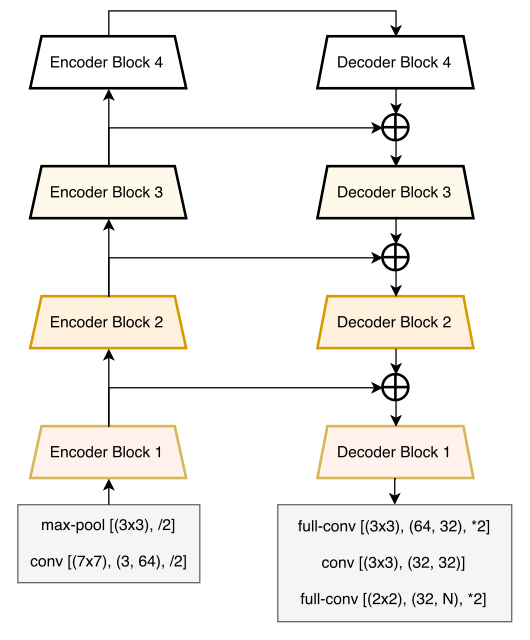
\includegraphics[width=0.35\textwidth]{./figures/linknet.png}
	\caption{High level description of the LinkNet model architecture \cite{DBLP:journals/corr/ChaurasiaC17}}
	\label{fig:linknet}
\end{figure}

Figure \ref{fig:linknet} shows a high level description of the model architecture. Network is constituted by two parts: an encoder and a decoder. The encoder is a residual net feature extractor. Decoder receives information from different feature maps of the encoder, summing up such values with their own. Figure \ref{fig:linknet_enc_dec} show a diagram with a high level description of encoder and decoder blocks. Instead of concatenating decoder and encoder values at the output of each layer, LinkNet uses a residual network approach summing up the values, ie. reducing the number of parameters of the final network.

\begin{figure}[h!]
    \centering
	\begin{subfigure}[t]{0.25\textwidth}
		\centering
			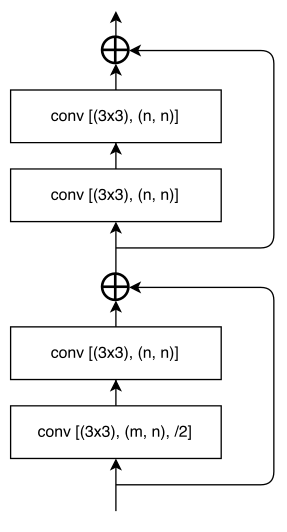
\includegraphics[width=0.5\textwidth]{./figures/linknet_encoder_block.png}
		\caption{Encoder block}
	\end{subfigure}%
	~ 
	\begin{subfigure}[t]{0.25\textwidth}
		\centering
		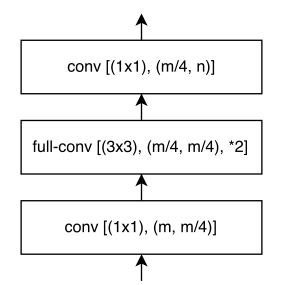
\includegraphics[width=0.5\textwidth]{./figures/linknet_decoder_block.png}
		\caption{Decoder block}
	\end{subfigure}	
	\caption{Encoder and Decoder blocks of LinkNet \cite{DBLP:journals/corr/ChaurasiaC17}}
	\label{fig:linknet_enc_dec}
\end{figure}

\section{Training procedure}
We split the training data in two sets: one with 13,000 images used for training and another one with 1,400 images for validation. We use the Adam optimizer with a learning rate of $10^-4$ and Dice coefficient as a loss function. Model with higher performance in the validation set is chosen as a final model.

\section*{References}

\bibliography{isic}

\end{document}